\documentclass{ximera}
\input{../preamble.tex}

\title{Challenge Problems for Ch 2} \license{CC BY-NC-SA 4.0}

\begin{document}

\begin{abstract}
\end{abstract}
\maketitle

\section*{Challenge Problems for Chapter 2}

\begin{problem}\label{prob:Anna3.1}
    Suppose $\{\vec{v}_{1}, \dots , \vec{v}_{m}\}$ is a linearly independent set in $\RR^n$, and that $\vec{w}$ is not in $\mbox{span}\left(\vec{v}_{1}, \dots , \vec{v}_{m}\right)$.

    \begin{enumerate}
        \item Is $\vec{w}$ in $\mbox{span}\left(\vec{v}_{1}+\vec{w}, \dots , \vec{v}_{m}+\vec{w}\right)$
        \wordChoice{\choice{YES}, \choice[correct]{NO}}

                \begin{hint}
            Suppose $\vec{w}$ is in $\mbox{span}\left(\vec{v}_{1}+\vec{w}, \dots , \vec{v}_{m}+\vec{w}\right)$.  Then we can write
\begin{align*}
    \vec{w} &= a_1 (\vec{v}_{1}+\vec{w}) + \dots + a_m (\vec{v}_{m}+\vec{w}) \\
    \vec{w} &= a_1\vec{v}_{1} + \dots + a_m\vec{v}_{m}+ (a_1 + \dots + a_m)\vec{w}.
    \end{align*}

Now consider two cases separately: either $a_1 + \dots + a_m = 0$ or $a_1 + \dots + a_m \ne 0$.  In either case, arrive at a contradiction and conclude that $\vec{w}$ is not in $\mbox{span}\left(\vec{v}_{1}+\vec{w}, \dots , \vec{v}_{m}+\vec{w}\right)$.
        \end{hint}

\item Is $\{\vec{v}_{1}+\vec{w}, \dots , \vec{v}_{m}+\vec{w}\}$ linearly independent?

\wordChoice{\choice[correct]{YES}, \choice{NO}}

\begin{hint}
            If you assume linear dependence, you should be able to show $\vec{w}$ is in the span of the original set, which is a contradiction.
\end{hint}

    \end{enumerate}
\end{problem}

\begin{problem}\label{prob:Anna3.2}
        Suppose $\vec{n}_1$, $\vec{n}_2$, and $\vec{n}_3$ are the rows of the $3 \times 3$ matrix $A$.  Then we can interpret the solution to the system of equations $[A|\vec{0}]$ as the intersection of three planes containing the origin.  Discuss what this intersection would look like geometrically if the reduced row echelon form of $[A|\vec{0}]$ is of the form:

\begin{enumerate}
\item
\begin{equation*}
\left[
\begin{array}{ccc|c}
1 & 0 & * & 0 \\
0 & 1 & * & 0 \\
0 & 0 & 0 & 0
\end{array}
\right]
\end{equation*}

\item
\begin{equation*}
\left[
\begin{array}{ccc|c}
1 & * & * & 0 \\
0 & 0 & 0 & 0 \\
0 & 0 & 0 & 0
\end{array}
\right]
\end{equation*}

\item  Are there any other possibilities?
            
\end{enumerate}
\end{problem}

\begin{problem}\label{prob:rowOfZeros}
    Show that for any matrix $A$, $\text{rref}(A)$ has a row of zeros if and only if one of the rows of $A$ can be expressed as a linear combination of the others.
\end{problem}

\begin{problem}\label{prob:normalVectInOnePlane}
    Recall that a plane in $\RR^3$ has an equation of the form $ax+by+cz=d$, where $a$, $b$, $c$ are the components of a normal vector to the plane.  Suppose three planes intersect in a line, as shown below.
    \begin{center}
\tdplotsetmaincoords{70}{130}
    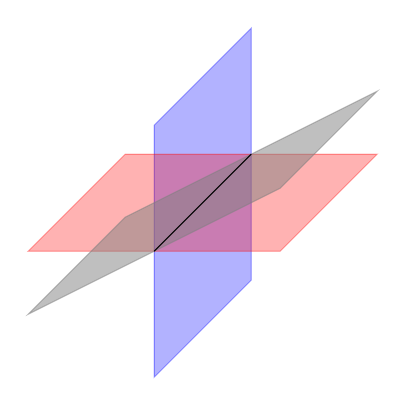
\begin{tikzpicture}[scale=0.8]
\filldraw[blue, opacity=0.3](0,-2,2)--(0,2,2)--(0,2,-2)--(0,-2,-2)--cycle;
\filldraw[red, opacity=0.3] (2,0,2)--(-2,0,2)--(-2,0,-2)--(2,0,-2)--cycle;
\filldraw[gray, opacity=0.5] (2,1,2)--(2,1,-2)--(-2,-1,-2)--(-2,-1,2)--cycle;
\draw[-](0,0,-2)--(0,0,2) ;
     \end{tikzpicture}
\end{center}     
We can find the line of intersection by solving a system of equations.  Suppose the augmented matrix $[A | \vec{d}]$ corresponds to this system.
\begin{enumerate}
    \item Explain why $\text{rref}[A | \vec{d}]$ will have a row of zeros.

\item Consider the normal vectors to the three planes.  What geometric property of these particular three normal vectors explains the row of zeros in the reduced row-echelon form?
\begin{hint}
    All three normal vectors lie in the same plane, so one of the normal vectors (rows) must be a linear combination of the other two.
\end{hint}
\end{enumerate}     
    

\end{problem}


\section*{Bibliography}
The first problem came from the end of Chapter 1 of Keith Nicholson's \href{https://open.umn.edu/opentextbooks/textbooks/linear-algebra-with-applications}{\it Linear Algebra with Applications}. (CC-BY-NC-SA)

W. Keith Nicholson, {\it Linear Algebra with Applications}, Lyryx 2018, Open Edition, pp. 33--34. 

\end{document}